\pdfminorversion=4
\documentclass[]{beamer}
\mode<presentation>
% Time-stamp: <2019-10-24 16:22:26 (jonahm)>

% beamer stuff
% Gives us the bottom line with all the goodies
\useoutertheme{infolines}
% Just the theme to use. Should be built into bemaer. Setting the
% height gets rid of a whole lot of whitespace
\usetheme[height=7mm]{Rochester}
\usefonttheme{serif}
% Usually beamer gives you navigation hyperlinks on the bottom
% right. I turned this off. It's annoying.
\setbeamertemplate{navigation symbols}{} 
% Makes my text boxes look pretty
\setbeamertemplate{blocks}[rounded][shadow=true] 
% Makes my bullet points 3d balls
\setbeamertemplate{items}[ball]

% Josh's packages
\usepackage{multimedia}
\usepackage{graphicx}

% Packages for me
\usepackage{amsmath,amssymb,latexsym,amsthm}
\usepackage[mathscr]{eucal}
\usepackage{mathrsfs}
\usepackage{verbatim}
\usepackage{braket}
\usepackage{listings}
\usepackage{xcolor}
% \usepackage[usenames,dvipsnames,svgnames,table]{xcolor}
\usepackage{fancybox}
\usepackage{animate}
% \usepackage{media9}
\usepackage{multicol}
\usepackage{mdframed}
\usepackage{hyperref}
%\usepackage{scalerel}
\usepackage[outline]{contour}
\contourlength{1.2pt}

% Macros

%Blackboard Bold
\newcommand{\R}{\mathbb{R}}
\newcommand{\Z}{\mathbb{Z}}
\newcommand{\N}{\mathbb{N}}
\newcommand{\Q}{\mathbb{Q}}
\newcommand{\A}{\mathbb{A}}
\newcommand{\E}{\mathbb{E}}
% other
\newcommand{\eval}{\biggr\rvert} %evaluated at
\newcommand{\myvec}[1]{\mathbf{#1}} % vectors for me
% total derivatives 
\newcommand{\diff}[2]{\frac{d #1}{d #2}} 
\newcommand{\dd}[1]{\frac{d}{d #1}}
% partial derivatives
\newcommand{\pd}[2]{\frac{\partial #1}{\partial #2}} 
\newcommand{\pdd}[1]{\frac{\partial}{\partial #1}} 
% Order operator
\DeclareRobustCommand{\orderof}{\ensuremath{\mathcal{O}}}

% braces
\newcommand{\paren}[1]{\left( #1 \right)}
\newcommand{\sqrbrace}[1]{\left[ #1 \right]}
\newcommand{\curlybrace}[1]{\left\{ #1 \right\}}
\newcommand{\inner}[1]{\paren{#1}}
\newcommand{\norm}[1]{\left| #1 \right|_2}

% g
\newcommand{\detg}{\sqrt{-g}}

% neutrinos
\newcommand{\eepsilon}{\epsilon} % energy
\newcommand{\fin}{f\in \{\nu_e,\nu_{\bar{e}},\nu_x\}}
\newcommand{\sign}{\text{sign}(f)}
\newcommand{\jnuf}{j_{\eepsilon,f}}
\newcommand{\etanuf}{\eta_{\eepsilon,f}}
\newcommand{\Inuf}{I_{\eepsilon,f}}
\newcommand{\chinuf}{\chi_{\eepsilon,f}}
\newcommand{\sigmanuf}{\sigma_{\eepsilon,f}}
\newcommand{\alphanuf}{\alpha_{\eepsilon,f}}
\newcommand{\numin}{\nu_{\text{min}}}
\newcommand{\numax}{\nu_{\text{max}}}


% tikz
\usepackage{tikz}
\usepackage{pgfplots}
\usetikzlibrary{arrows}
\usetikzlibrary{decorations.pathmorphing}

% Keys to support piece-wise uncovering of elements in TikZ pictures:
% \node[visible on=<2->](foo){Foo}
% \node[visible on=<{2,4}>](bar){Bar}   % put braces around comma expressions
% 
% Internally works by setting opacity=0 when invisible, which has the 
% adavantage (compared to \node<2->(foo){Foo} that the node is always there, hence
% always consumes space plus that coordinate (foo) is always available.
% 
% The actual command that implements the invisibility can be overriden
% by altering the style invisible. For instance \tikzsset{invisible/.style={opacity=0.2}}
% would dim the "invisible" parts. Alternatively, the color might be set to white, if the
% output driver does not support transparencies (e.g., PS) 
% 
\tikzset{
  invisible/.style={opacity=0},
  visible on/.style={alt={#1{}{invisible}}},
  alt/.code args={<#1>#2#3}{%
    \alt<#1>{\pgfkeysalso{#2}}{\pgfkeysalso{#3}} % \pgfkeysalso doesn't change the path
  },
}

% some nice flowchart features
\tikzset{
    mynode/.style={rectangle,rounded corners,draw=black, top color=white, bottom color=yellow!50,very thick, inner sep=1em, minimum size=3em, text centered},
    myarrow/.style={->, >=latex', shorten >=1pt, thick},
    mylabel/.style={text width=7em, text centered} 
}  

% squigly arrow
\tikzset{zigzag it/.style={decorate, decoration=zigzag}}

% define a really nice visible "purple"
\definecolor{gimppurple}{HTML}{AD26FB}
% a light grey
\definecolor{lightgrey}{HTML}{E0E0E0}
% for highlighting
\definecolor{deepblue}{rgb}{0,0,0.5}
\definecolor{deepred}{rgb}{0.6,0,0}
\definecolor{deepgreen}{rgb}{0,0.5,0}

% fonts
% Default fixed font does not support bold face
\DeclareFixedFont{\ttb}{T1}{txtt}{bx}{n}{12} % for bold
\DeclareFixedFont{\ttm}{T1}{txtt}{m}{n}{12}  % for normal

% Python style for highlighting
\newcommand\pythonstyle{\lstset{
language=Python,
basicstyle=\ttm,
otherkeywords={self},
keywordstyle=\ttb\color{deepblue},
emph={__init__},           
emphstyle=\ttb\color{deepred},
commentstyle=\ttfamily\color{deepred},
stringstyle=\color{deepgreen},
frame=tb,                     
showstringspaces=false        
}}

% Python environment
\lstnewenvironment{python}[1][]
{
\pythonstyle
\lstset{#1}
}
{}

\newcommand{\backupbegin}{
   \newcounter{finalframe}
   \setcounter{finalframe}{\value{framenumber}}
}
\newcommand{\backupend}{
   \setcounter{framenumber}{\value{finalframe}}
}

% Automatically generates section breaker slides
\AtBeginSection[]{
  \begin{frame}[plain]
  \vfill
  \centering
  \begin{beamercolorbox}[sep=8pt,center,shadow=true,rounded=true]{title}
    \usebeamerfont{title}\insertsectionhead\par%
  \end{beamercolorbox}
  \vfill
  \end{frame}
}

\title[DR Review]{Neutrino Transport and Nucleosynthesis in Post-Merger Disks}
% \subtitle{Models and Implications}
\author[J. Miller]{\textcolor{blue}{Jonah M. Miller},\\B. Ryan, J. Dolence\\
  A. Burrows, C. Fryer, C. Fontes,\\
  O. Korobkin,  J. Lippuner, \\
  M. Mumpower, T. Sprouse,\\
  R. Surman, R. Wollaeger,\\
  More...}
\institute[LANL]{Los Alamos National Laboratory}
% \titlegraphic{\vspace{1cm}}
% \titlegraphic{\includegraphics[height=0.25\textheight]{3d_render}}
\date[12/09/19]{DR Review}

\graphicspath{{figures/}}

\begin{document}

\begin{frame}[plain]
    \tikz [remember picture, overlay] 
    \node at ([xshift=2cm,yshift=-2cm]current page.west)
    {\includegraphics[width=0.25\textwidth,clip,trim={150 0 150 0}]{3d_render}};
    \tikz [remember picture, overlay] 
    \node at ([xshift=-2cm,yshift=-2cm]current page.east)
    {\includegraphics[width=0.25\textwidth,clip,trim={0 0 0 0}]{visit0006-gimp3}};
  \titlepage
\end{frame}

\begin{frame}
  \frametitle{Neutron Star Mergers: A 2+ Component Model}
  \begin{columns}
    \begin{column}{6cm}
      \begin{center}
        % \includegraphics[width=0.9\textwidth]{frames/betabin_000}
        \animategraphics[width=0.9\textwidth,every=10,autoplay,loop,controls]
        {5}{frames/betabin_}{000}{374}
      \end{center}
    \end{column}
    \begin{column}{6cm}
      \begin{center}
        \resizebox{\columnwidth}{!}{
          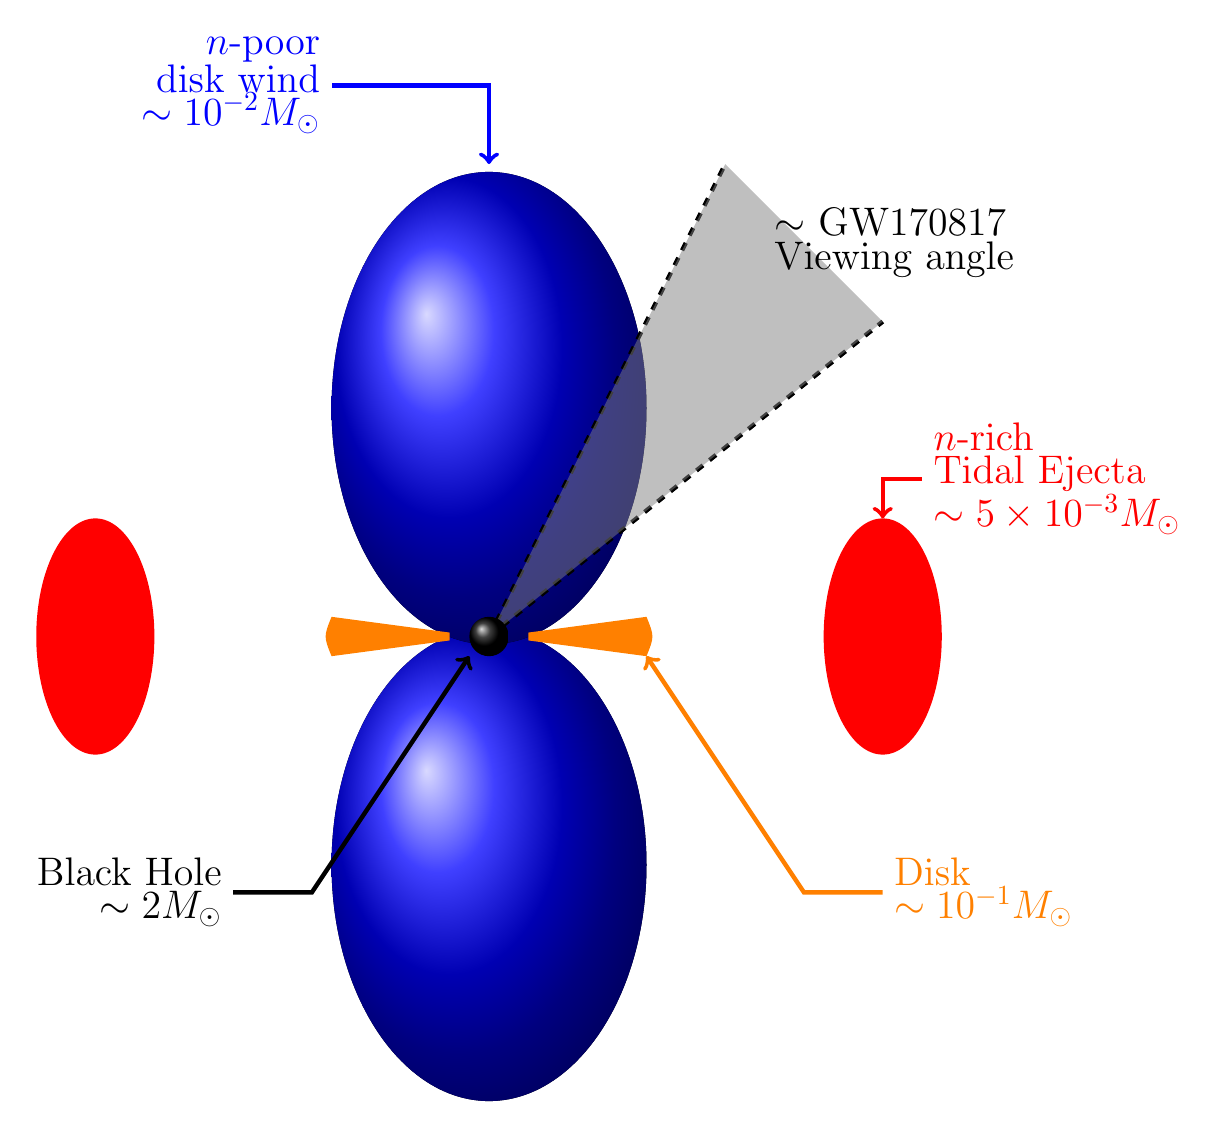
\begin{tikzpicture}
            \coordinate (origin) at (0,0);
            \pgfmathsetmacro{\dbx}{0.5}
            \pgfmathsetmacro{\dby}{0.05}
            \pgfmathsetmacro{\dex}{2.}
            \pgfmathsetmacro{\dey}{0.25}
            \pgfmathsetmacro{\dcc}{2.1}
            \pgfmathsetmacro{\tcx}{5.0}

            \foreach \i in {-1,1}
            {
              \fill[ball color=blue] (0, \i*2.9) ellipse (2 and 3);
            }

            \foreach \i in {-1,1}
            {
              % disk
              \fill[color=orange]
              (\i*\dbx,\dby) -- (\i*\dex,\dey)
              .. controls (\i*\dcc,0) .. (\i*\dex,-\dey)
              -- (\i*\dbx,-\dby) -- cycle;

              % tidal ejecta
              \fill[color=red] (\i*\tcx,0) ellipse (0.75 and 1.5);
            }

            % viewing
            \draw[dashed,ultra thick,black] (origin) -- (5,4);
            \draw[dashed,ultra thick,black] (origin) -- (3,6);
            \fill[color=gray,opacity=0.5] (origin) -- (5,4) -- (3,6) -- cycle;
            \node[right,align=left] at (3.5,5)
            {\Large $\sim$ GW170817\\ \Large Viewing angle};

            % bh
            \shade[ball color=black] (origin) circle (0.25);

            % text
            \draw[<-,red, ultra thick] (\tcx,1.5)
            -- ++(0.,0.5) -- ++(0.5,0)
            node[right,align=left]
            {\Large \color{red}$n$-rich\\\Large Tidal Ejecta\\ \Large $\sim 5\times 10^{-3}M_{\odot}$};

            \draw[<-,blue, ultra thick] (0,6) -- ++(0,1) -- ++(-2,0)
            node[left,align=right]
            {\Large \color{blue}$n$-poor\\\Large disk wind\\\Large $\sim 10^{-2}M_{\odot}$};

            \draw[<-,orange, ultra thick] (\dex,-\dey)
            -- ++(2,-3) -- ++(1,0)
            node[right,align=left]
            {\Large \color{orange}Disk\\\Large $\sim 10^{-1}M_{\odot}$};

            \draw[<-,black, ultra thick] (-0.25,-0.25)
            -- ++(-2,-3) -- ++(-1,0)
            node[left,align=right]
            {\Large \color{black}Black Hole\\ \Large $\sim 2 M_{\odot}$};
          \end{tikzpicture}
        }
      \end{center}
    \end{column}
  \end{columns}
  \begin{tiny}
    Co-design summer school, 2016
  \end{tiny}
\end{frame}

\begin{frame}
 \frametitle{The r-process}
 \begin{center}
  \includegraphics[width=0.9\textwidth]{skynet_ye_0p13/frame_0001}
 \end{center}
 Courtesy of J. Lippuner
\end{frame}

\begin{frame}
 \frametitle{The r-process}
 \begin{center}
   % \includegraphics[width=0.9\textwidth]{skynet_ye_0p13/frame_0001}
   \animategraphics[width=0.9\textwidth,every=5,autoplay,loop,controls]
   {5}{skynet_ye_0p13/frame_}{0001}{0108}
 \end{center}
 Courtesy of J. Lippuner
\end{frame}

\begin{frame}
  \frametitle{Opacity}
  %\setlength{\unitlength}{1cm}
  \resizebox{12cm}{!}{
    \begin{tikzpicture}
      \node[inner sep=0pt] (rp) at (0,0)
      {\includegraphics[width=10cm]{skynet_ye_0p13/frame_0108}};
      \draw[ultra thick,red,<-] (1.5,-2) -- (2,-2.85)
      -- (2.25, -2.85) node[right] {\tiny Opaque to visible light};
      \draw[ultra thick,red,<-] (0.85,-2) -- (0.5,-2.85)
      -- (0.25,-2.85) node[left] {\tiny Not opaque};
    \end{tikzpicture}
  }
\end{frame}

\begin{frame}
  \frametitle{The Kilonova}
  \begin{center}
    \includegraphics[width=10cm]{swope-image}
  \end{center}
  M2H/UC Santa Cruz and Carnegie Observatories/Ryan Foley
\end{frame}

% \begin{frame}
%   \frametitle{Time Scales}
%   \begin{itemize}
%   \item In-spiral: $\sim$ 30 s
%   \item Disk + GRB: $\sim$ 1 s
%   \item Nucleosyntheis: $\sim$ hours
%   \item Kilonova: Weeks
%   \end{itemize}
% \end{frame}

\begin{frame}
  \frametitle{Lets Focus on the Disk}
  \begin{center}
    \resizebox{12.cm}{!}{
      \begin{tikzpicture}
        \filldraw[black] (0,0) rectangle ++(12,8);
        % \node[right,align=left] at (0,0.25){\color{red}\textbf{JMM}+, in prep.};
        \node[inner sep=0pt] (wind) at (3,4)
        {\includegraphics[width=0.5\textwidth]{wind-3d-render}};
        \node[inner sep=0pt,rectangle,blue,ultra thick] (disk) at (9,5)
        {\includegraphics[width=0.4\textwidth]{disk_image_no_text}};
        \draw[blue,ultra thick] (6.5,3.5) rectangle ++(5,3.);
        \draw[blue,ultra thick] (3,4) -- (6.5,6.5);
        \draw[blue,ultra thick] (3,4) -- (6.5,3.5);
      \end{tikzpicture}
      %\includegraphics[width=7cm]{disk_3d_render}
      }
  \end{center}
\end{frame}

\begin{frame}
  \frametitle{Neutrino Transport Matters!}
  \begin{center}
    % \includegraphics[height=0.8\textheight]{leptoneq/frame_0001}
    \animategraphics[height=0.8\textheight,every=5,autoplay,loop,controls]
    {5}{leptoneq/frame_}{0001}{0101}
  \end{center}
  \begin{tiny}
    \textbf{JMM}, B. R. Ryan, J. C. Dolence. ApJS \textbf{241} 30 (2019) 
  \end{tiny}
\end{frame}

% \begin{frame}
%   \frametitle{Accretion Rates}
%   \begin{center}
%     \includegraphics[width=0.9\textwidth]{mdot_edd}
%   \end{center}
% \end{frame}
% 
% \begin{frame}
%   \frametitle{Accretion Rates}
%   \begin{center}
%     \includegraphics[width=0.9\textwidth]{mdot_edd_nu}
%   \end{center}
% \end{frame}

\begin{frame}
  \frametitle{Ingredients In Kilonova Disk Modeling}
  \begin{itemize}
  \item General relativity
    \begin{itemize}
    \item Rotating black hole spacetime
    \end{itemize}
  \item Plasma physics
    \begin{itemize}
    \item Ideal magnetohydrodynamics
    \end{itemize}
  \item Nuclear physics
    \begin{itemize}
    \item Hot gas treated as being in nuclear-statistical equilibrium via \textbf{equation of state}
    \item Cooling outflow treated in postprocessing via \textbf{nuclear reaction networks}
    \end{itemize}
  \item Radiation physics
    \begin{itemize}
    \item Material is opaque to photons, can be incorporated in plasma physics
    \item Material \textit{not} opaque to \textbf{neutrinos}.
    \item Neutrinos can \textit{change the composition of the
        material} by converting neutrons to protons and vice versa.
    \end{itemize}
  \end{itemize}
\end{frame}

% \begin{frame}
%   \frametitle{Ingredients in Kilonova Disk Modeling}
%   \begin{itemize}
%   \item Mass conservation:
%     \begin{small}
%       \begin{displaymath}
%         \partial_t \paren{{\color{red}\detg}\rho_0 u^t}
%         + \partial_i\paren{{\color{red}\detg}\rho_0u^i} = 0
%       \end{displaymath}
%     \end{small}
%   \item Momentum and Internal Energy Conservation:
%     \begin{small}
%       \begin{displaymath}
%         \partial_t\sqrbrace{{\color{red}\detg} \paren{T^t_{\ \nu} + \rho_0u^t \delta^t_\nu}}
%         + \partial_i\sqrbrace{{\color{red}\detg}\paren{T^i_{\ \nu} + \rho_0 u^i \delta^t_\nu}}
%         = {\color{red}\detg} \paren{T^\kappa_{\ \lambda} {\color{red}\Gamma^\lambda_{\nu\kappa}} + {\color{blue}G_\nu}}
%       \end{displaymath}
%     \end{small}
%   \item Magnetic Fields
%     \begin{small}
%       \begin{displaymath}
%         \partial_t \paren{{\color{red}\detg} B^i}
%         - \partial_j \sqrbrace{{\color{red}\detg}\paren{b^ju^i - b^i u^j}}
%         = 0
%       \end{displaymath}
%     \end{small}
%   \item Composition
%     \begin{small}
%       \begin{displaymath}
%         \partial_t\paren{{\color{red}\detg}\rho_0 Y_e u^t}
%         + \partial_i\paren{{\color{red}\detg}\rho_0Y_eu^i}
%         = {\color{red}\detg} {\color{blue}G_{\text{ye}}}
%       \end{displaymath}
%     \end{small}
%   \item Neutrino Transport
%     \begin{small}
%       \begin{displaymath}
%         {\color{red}\frac{D}{d\lambda}}\paren{\frac{h^3\Inuf}{\eepsilon^3}}
%         = \paren{\frac{h^2{\color{blue}\etanuf}}{\eepsilon^2}}
%         - \paren{\frac{\eepsilon {\color{blue}\chinuf}}{h}} \paren{\frac{h^3\Inuf}{\eepsilon^3}},
%       \end{displaymath}
%     \end{small}
%   \end{itemize}
% \end{frame}

\begin{frame}
  \frametitle{Presenting $\nu\texttt{bhlight}$!}
  \begin{itemize}
  \item General relativistic radiation magnetohydrodynamics for kilonova disks
  \item \textbf{Magnetized gas} via \textit{finite volume methods}
    \begin{itemize}
    \item Standard second-order Gudonov scheme
    \item Cell-centered constrained transport for magnetic fields
    \item WENO5 reconstruction
    \item Local Lax-Friedrichs Riemann solver
    \end{itemize}
  \item \textbf{Neutrinos} via \textit{Monte Carlo methods}
    \begin{itemize}
    \item Explicit integration along geodesics
    \item Probabilistic emissivity, absorption, and scattering
    \item Novel biasing scheme ensures all processes well-sampled
    \end{itemize}
  \item \textbf{Coupled} via \textit{operator splitting}
  \item Built on top of $\texttt{HARM}$, $\texttt{grmonty}$, and
    $\texttt{bhlight}$.
  \end{itemize}
\end{frame}

\begin{frame}
  \frametitle{The August 2017 Disk}
  \begin{center}
    % \includegraphics[height=0.475\textheight]{gw170817disk_Ye_close/frame_0831} \\
    % \includegraphics[height=0.475\textheight]{gw170817disk_Ye_far/frame_0831} 
    \animategraphics[height=0.475\textheight,every=5,autoplay,loop,controls=off]
    {10}{gw170817disk_Ye_close/frame_}{0001}{0837} \\
    \animategraphics[height=0.475\textheight,every=5,autoplay,loop,controls=off]
    {10}{gw170817disk_Ye_far/frame_}{0001}{0837} 
  \end{center}
  %\textbf{JMM}+, in prep.
\end{frame}

% \begin{frame}
%   \frametitle{Neutrino Transport}
%   \begin{center}
%     % \includegraphics[height=0.9\textheight]{tau_frames/frame_00531}
%     \animategraphics[height=0.9\textheight,every=10,autoplay,loop,controls=off]
%     {20}{tau_frames/frame_}{00001}{00983}
%   \end{center}
% \end{frame}

\begin{frame}
  \frametitle{Neutrino Transport}
  \begin{center}
    % \includegraphics[width=0.9\textwidth]{nphys_frames/frame_00531}
    \animategraphics[width=0.9\textwidth,every=10,autoplay,loop,controls=off]
    {20}{nphys_frames/frame_}{00001}{00965}
  \end{center}
  \begin{tiny}
    \textbf{JMM} et al. PRD \textbf{100} 023008 (2019)
  \end{tiny}
\end{frame}

\begin{frame}
  \frametitle{Electron Fraction}
  \setlength{\unitlength}{1cm}
  \begin{picture}(12,8)
    \visible<1>{
      \put(2,1){
        \includegraphics[width=8cm]{gw170817-log-divergence-dyedt-tavg-wb}
      }
    }
    \visible<2->{
      \put(6,4){
        \includegraphics[height=4cm]{gw170817-log-divergence-dyedt-tavg-wb}
      }
      \put(0,0.5){
        \includegraphics[height=0.9\textheight]{gw170817-ye-vs-theta-folded-5}
      }
    }
    \visible<3->{
      \put(6,0.5){
        \includegraphics[width=5.5cm]{gw170817-yields-2}
      }
    }
    \visible<1->{
      \put(0,0){
        \begin{tiny}
          \textbf{JMM} et al. PRD \textbf{100} 023008 (2019)
        \end{tiny}
      }
    }
  \end{picture}
\end{frame}

\begin{frame}
  \frametitle{Light Curves}
  \begin{center}
    \includegraphics[width=0.9\columnwidth]{spectral_evolution}
  \end{center}
  \begin{tiny}
    \textbf{JMM} et al. PRD \textbf{100} 023008 (2019)
  \end{tiny}
\end{frame}

\begin{frame}
  \frametitle{Open Questions}
  \begin{columns}
    \begin{column}{7cm}
      \begin{itemize}
      \item How generic are these results?
        \begin{itemize}
        \item Hypermassive NS?
        \item Neutrino annihilation and the jet
        \item Black Hole-Neutron Star Mergers?
        \item Initial data?
        \item Collapsars? (on ArXiv tomorrow!)
        \item Oscillations? Neutral current excitations?
        \end{itemize}
      \item Pipeline ties
        \begin{itemize}
        \item Nuclear physics
        \item MultiD radiation transport
        \end{itemize}
      \item Physics questions (in prep.):
        \begin{itemize}
        \item What launches the wind?
        \item What macroscopic quantities set electron fraction?
        \end{itemize}
      \end{itemize}
    \end{column}
    \begin{column}{5cm}
      \begin{center}
        \includegraphics[height=0.5\textheight]{gw170817/gain_vs_loss_time_inst}\\
        \includegraphics[width=0.9\columnwidth]{gw170817/force_vectors_gr}
      \end{center}
    \end{column}
  \end{columns}
\end{frame}

% \begin{frame}
%   \frametitle{Electron Fraction}
%   \begin{columns}
%     \begin{column}{6cm}
%       \begin{center}
%         \includegraphics[height=0.9\textheight]{gw170817-ye-vs-theta-folded-5}
%       \end{center}
%     \end{column}
%     \begin{column}{6cm}
%       \includegraphics[width=0.9\columnwidth]{gw170817-log-divergence-dyedt-tavg-wb}\\
%       \includegraphics[width=0.9\columnwidth]{gw170817-yields-2}
%     \end{column}
%   \end{columns}
%   \begin{tiny}
%       \textbf{JMM} et al. PRD \textbf{100} 023008 (2019)
%   \end{tiny}
% \end{frame}



\begin{frame}
  \frametitle{Conclusions}
  \begin{columns}
    \begin{column}{6cm}
      \begin{itemize}
      \item Need GRRMHD and neutrino transport!
      \item NS Mergers:
        \begin{itemize}
        \item Likely source of heavy elements in our
          universe
        \item Preliminary results show disks can produce blue component of
          kilonova
        \end{itemize}
      \item Many open questions:
        \begin{itemize}
        \item Extending results to more systems, both merger and collapsar
        \item Better understanding the physics in these systems
        \end{itemize}
      \item Lots of exciting stuff to do!
      \end{itemize}
    \end{column}
    \begin{column}{6cm}
      \includegraphics[width=\columnwidth,clip,trim={150 0 150 0}]{3d_render}
    \end{column}
  \end{columns}
\end{frame}

\backupbegin
\backupend

\end{document}